\chapter{Sincronização}

A sincronização do sinal adquirido de diferentes equipamentos pode ser um desafio 
(Tu et al., 2020). Algumas propostas já foram exploradas a respeito, 
como o uso sincronização temporal e sincronização por piscadas (Xiao et al., 2022, 
Bækgaard et al. 2015, Notaro et al. 2018). Outra solução
conta com o disparo de pulsos para os equipamentos de coleta fisiológica 
(Baccino e Manunta, 2005) e posterior sincronização. 


\section{Sincronização com Timecode}
Notaro et al. (2018) fez uma integração de equipamentos de coleta fisiológica e comportamental de 
baixo custo, através do equipamento OpenBCI para captura de EEG; GP3 para ET e dados 
de movimentação do mouse em tela. Os dados foram coletados enquanto os partipantes realizavam atividades em um 
site de línguas. Os dados de EEG foram coletados em frequencia de 250Hz e dados de ET e deslocamento
do mouse foram gravados em 60 Hz. Em sua pesquisa, Norato et al.  faz uso uso do código temporal, ou \textit{timecode}, 
para sincronizar as diferentes modalidades. 

O driver do fabricante do equipamento 
comercial de EEG utilizado permite alteração da latência da coleta de dados, que
foi modificada do valor padrão de 16 milissegundos para 1 millisegundo, afim de aumentar a precisão do 
equipamento. A granularidade do \textit{timecode} foi de milissegundos (HH:MM:SS:MsMsMs), informação posteriormente utilizada
para montar uma base de dados onde é possível identificar ondas cerebrais e coordenada do foco ocular em tela (figura 6.1). 
A calibração do GP3 e coleta de dados de ET foi realizada através de código desenvolvido em Python, enquanto a
coleta de EEG é realizada por software próprio do OpenBCI e posteriormente unida em código em MATLAB, onde os dados são
sincronizados para poder gerar imagens como a do exemplo abaixo. 


\begin{figure}[!h]
    \centering
    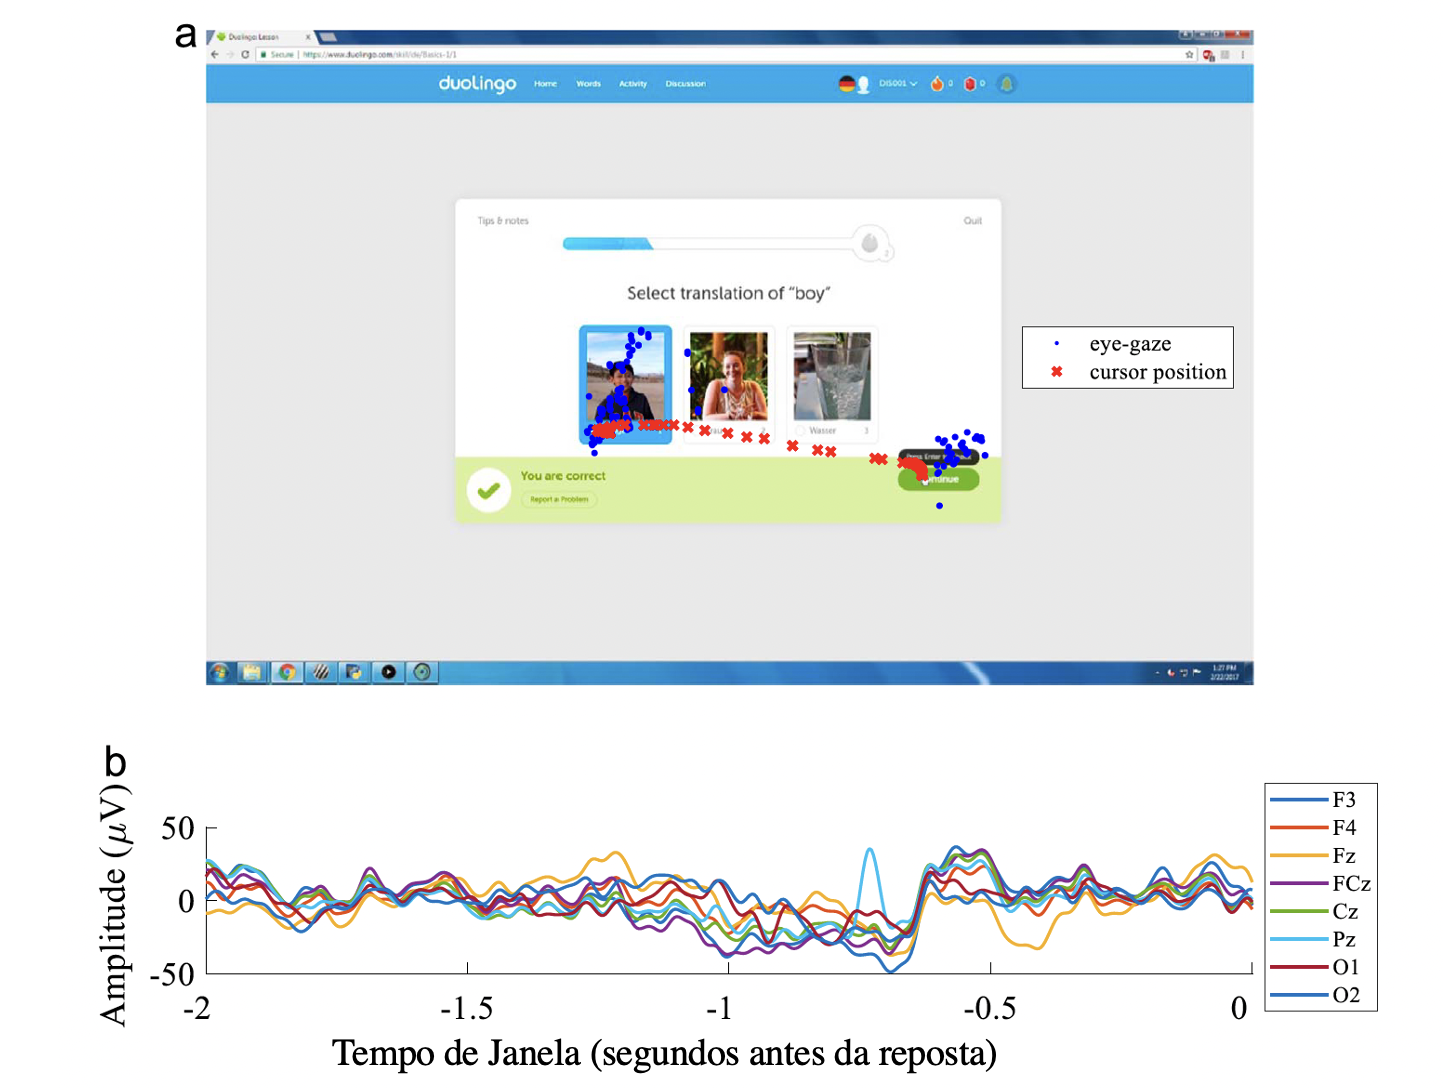
\includegraphics[width=180mm]{Screen Shot 2022-08-15 at 22.11.48.png}
    \caption{Dados de EEG, ET (eye gaze) e posição de cursor (cursor position) 2 segundos antes da resposta de um participante em atividades de um site de línguas. 
    Fonte: Notaro et al. (2018).}
\end{figure}

\clearpage

\section{Sincronização com Piscadas}
Piscadas duram cerca de 200 milissegundos em média, com o tempo de abertura 
das pálpebras sendo cerca de duas vezes mais longo que a duração 
do fechar das pálpebras (Caffier et al., 2013). O comportamento de piscar também tende a 
ser relaicionado a condições de alerta e a depender se 
o participante está engajado de forma ativa ou assistindo de forma 
passiva a determinada atividade  (Caffier et al., 2013; Skotte et al. 2007). 


e aparecem em 
sinais de EEG de forma característica, 
podendo alcançar uma amplitude de sinal acima de 200 microvolts em eletrodos próximos a 
órbita ocular (Hoffmann e Falkenstein, 2008). Assim sendo, é possível realizar uma sincronização 
por piscadas ao se detectar o movimento em ambos os equipamentos de coleta. 
No caso do EEG, as piscadas são comumente descartadas como artefatos indesejáveis. 
Já no estudo de Bækgaard et al. (2015), elas são a assinatura de sincronização 
entre os equipamentos de coleta de EEG e ET em função de sua onda característica
 (geralmente muitos milivolts acima do sinal do EEG), e de também 
ser detectada através dos equipamentos de rastreamento ocular.






A piscada envolve ativação muscular, e o dipolo ocular também influencia na captura de alterações de voltagem em eletrodos próximos aos olhos
(Croft e Barry, 2000). Seu reflexo no EEG pode ser facilmente identificado pois tente a ter uma amplitude e forma de sinal característicos. 
A amplitude de uma atividade de piscada no sinal de EEG tem uma média de 200 microvolts (Hoffmann et al., 2008). Esta característica permite
que o poder elétrico somado de eletrodos de interesse possam auxiliar na determinação de uma probabilidade do evento capturado ser uma piscada. 
No estudo de Bækgaard et al. (2015), as assinaturas de piscadas foram alinhadas entre as modalidades de EEG e ET para garantir a sincronizaçã, e
o começo da atividade de piscada (com o fechamento das pálpebras) foi eleito como o ponto de referencia da assinatura. 


Para se detectar a piscada através de um sinal, é possível tentar realizar o método de \textit{Independent Component Analysis}, ou análise de 
componente independente, mas as características do sinal de piscada também permite outras abordagens, como a identificação por função de probabilidade.

EEG-Blinks é uma \textit{toolbox} feita para MATLAB que possibilita a coleta de piscadas em dados de EEG, que 
funciona primeiramente extraindo possíveis sinais de piscadas do sinal de EEG, calculando pontos de interesse (figura 6.1) 
nos sinais potenciais sinais de piscadas, rejeitando sinais com baixo SNR, e calculando o melhor sinal de piscada
para ser utilizado. A partir disso, ele calcula as propriedades do sinal de piscada e seus índices (Blinker, 2022).

\begin{figure}[!h]
    \centering
    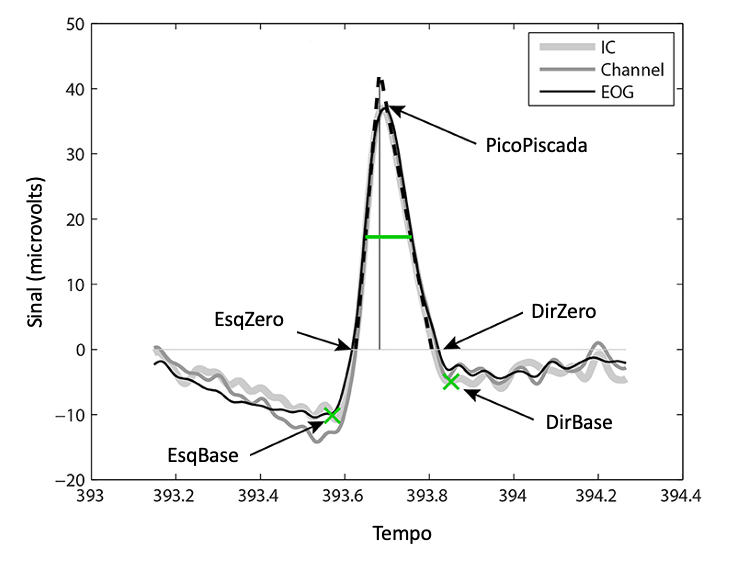
\includegraphics[width=100mm]{blink.png}
    \caption{Assinatura de piscada em microvolts. Fonte: Blinker (2022)}
\end{figure}
 


Como o equipamento de rastreamento procura encontrar sinais da movimentação ocular, ele também detecta a ausencia desse sinal. No estudo 
de Bækgaard et al. (2015), uma perda de até 500 milissegundos foi considerada como indicador da ocorrência de uma piscada. No equipamento de coleta de ET GP3, 
o fabricante oferece uma forma de identificar a existencia de uma piscada. Ela ocorre através da propriedade Blinking Validation Flag, ou BKID, onde qualquer 
valor diferente de 0 indica ocorrência de piscada durante o timeframe. A extração de piscada através do BKID foi utilizada no estudo de Seha et al. (2019), 
onde o blink rate foi validado e sincronizado com o vídeo do próprio equipamento (que indica quando houve piscada através da ausencia da imgem dos olhos do usuário).



\section{Calcular a Sincronização}
Existem diferentes métodos para calculo de sincronização entre séries temporais. 
A forma mais simples é por \textbf{correlação de Pearson}, que mede como dois sinais mudam ao longo do tempo em valores que vão de -1 a 1;
com -1 indicando uma correlação perfeita e negativa, 1 uma correlação perfeita e 0, sem correlação. 
É importante notar que anomalias vão impactar significativamente a correlação, e que os dados assumem que a variância é homogênea. 

Outro método de sincronização entre séries temporais é o \textit{\textbf{lag cross-correlation}}, onde é possível identificar
qual sinal vem primeiro. A correlação é calculada através da mudança gradual de um vetor de série temporal e subsequente cálculo 
de correlação. A correlação cruzada procura calcular a similaridade entre dois sinais com a aplicação de um \textit{delay} em apenas um dos sinais.

Um exemplo de seu uso é no trabalho de Com dois sinais diferentes em EEG e ET, Bækgaard et al. (2015) opta por correlacionar as funções de probabilidade do evento observado em 
ambos os equipamentos, ser uma piscada. 
Para correlacionar assinaturas diferentes, as probabilidades de ocorrencia de um evento (piscada) em duas séries temporais são convertidas em uma mesma frequência amostral (Bækgaard et al., 2014).
A similatidade entre sinais é medida na amplitude do sinal da correlação. A correlação cruzada é definida como:
\begin{equation}\label{eq:correlação cruzada}
    (f * g) = f(-t)*g(t), 
    \end{equation}
onde * significa convolução e f(-t) é o conjugado complexo de f(t).

